% Frozen evidence: manuscript/evidence/2026-10-22/polymer_validation.json
\begin{frame}{A nearby graft changes the next attachment free energy}
\centering
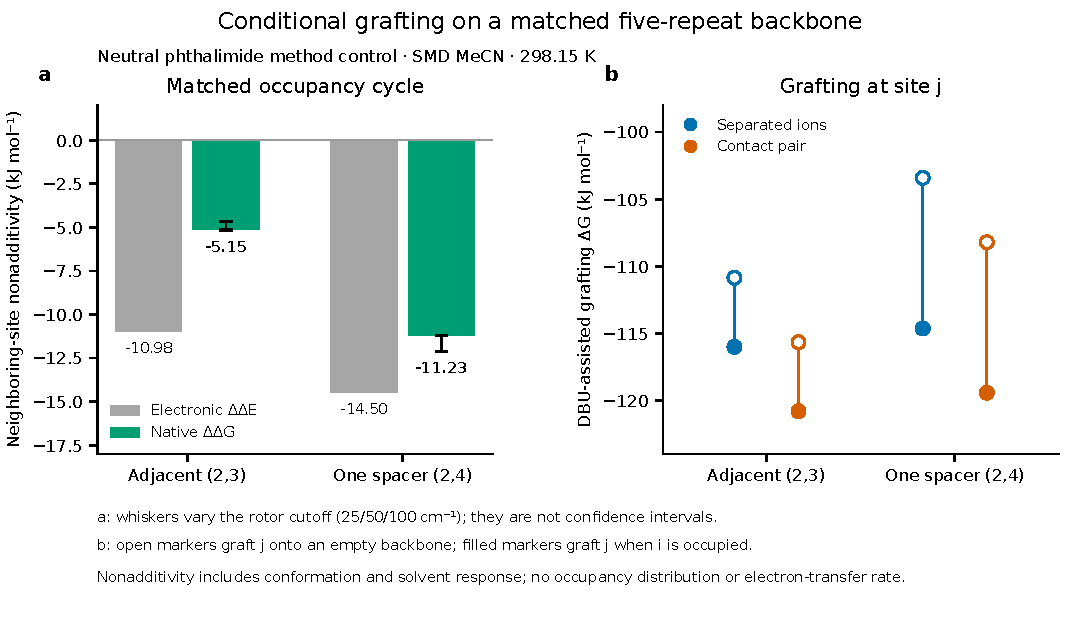
\includegraphics[width=.95\linewidth,height=.70\textheight,keepaspectratio]{../results/figures/manuscript/2026-10-22/conditional_grafting.pdf}
\par\smallskip\small
Six selected native free energies pass QC. Neighbor effects include conformation and solvent.
\par\footnotesize Phthalimide control; two conformers per graph. No general spacing rule, occupancy probability or electron-transfer rate.
\end{frame}
\begin{frame}{Route thermodynamics still needs quantitative validation}
\begin{block}{A defined term exposes model sensitivity}
For DBU + HCl $\rightarrow$ DBUH$^+$ + Cl$^-$ in MeCN:
\begin{center}
\begin{tabular}{lr}
\toprule
Capture model & $\Delta G$ (kJ/mol)\\
\midrule
Computed separated ions & $-102.78$\\
Author-tabulated pKa anchors at 298.15 K & $-79.97$\\
Difference & $-22.81$\\
\bottomrule
\end{tabular}
\end{center}
\end{block}
\small Exact source temperature/activity conventions remain under review. HCl cancels from the full all-DFT grafting cycle; changing only this term changes shared-error cancellation.
\par\medskip\textcolor{teal}{\textbf{Both BQ signs survive the limited DBU term sensitivity. Full grafting accuracy remains unvalidated.}}
\par\vfill\scriptsize Sources: Leito-group tables; DOI 10.1002/ejoc.201900956 and 10.1002/poc.2946. No exact DIPEA anchor substituted.
\end{frame}
